\documentclass{article}

\usepackage{graphicx}
\usepackage{tikz-cd}
\usepackage[margin=0.25in]{geometry}

\begin{document}

\begin{center}
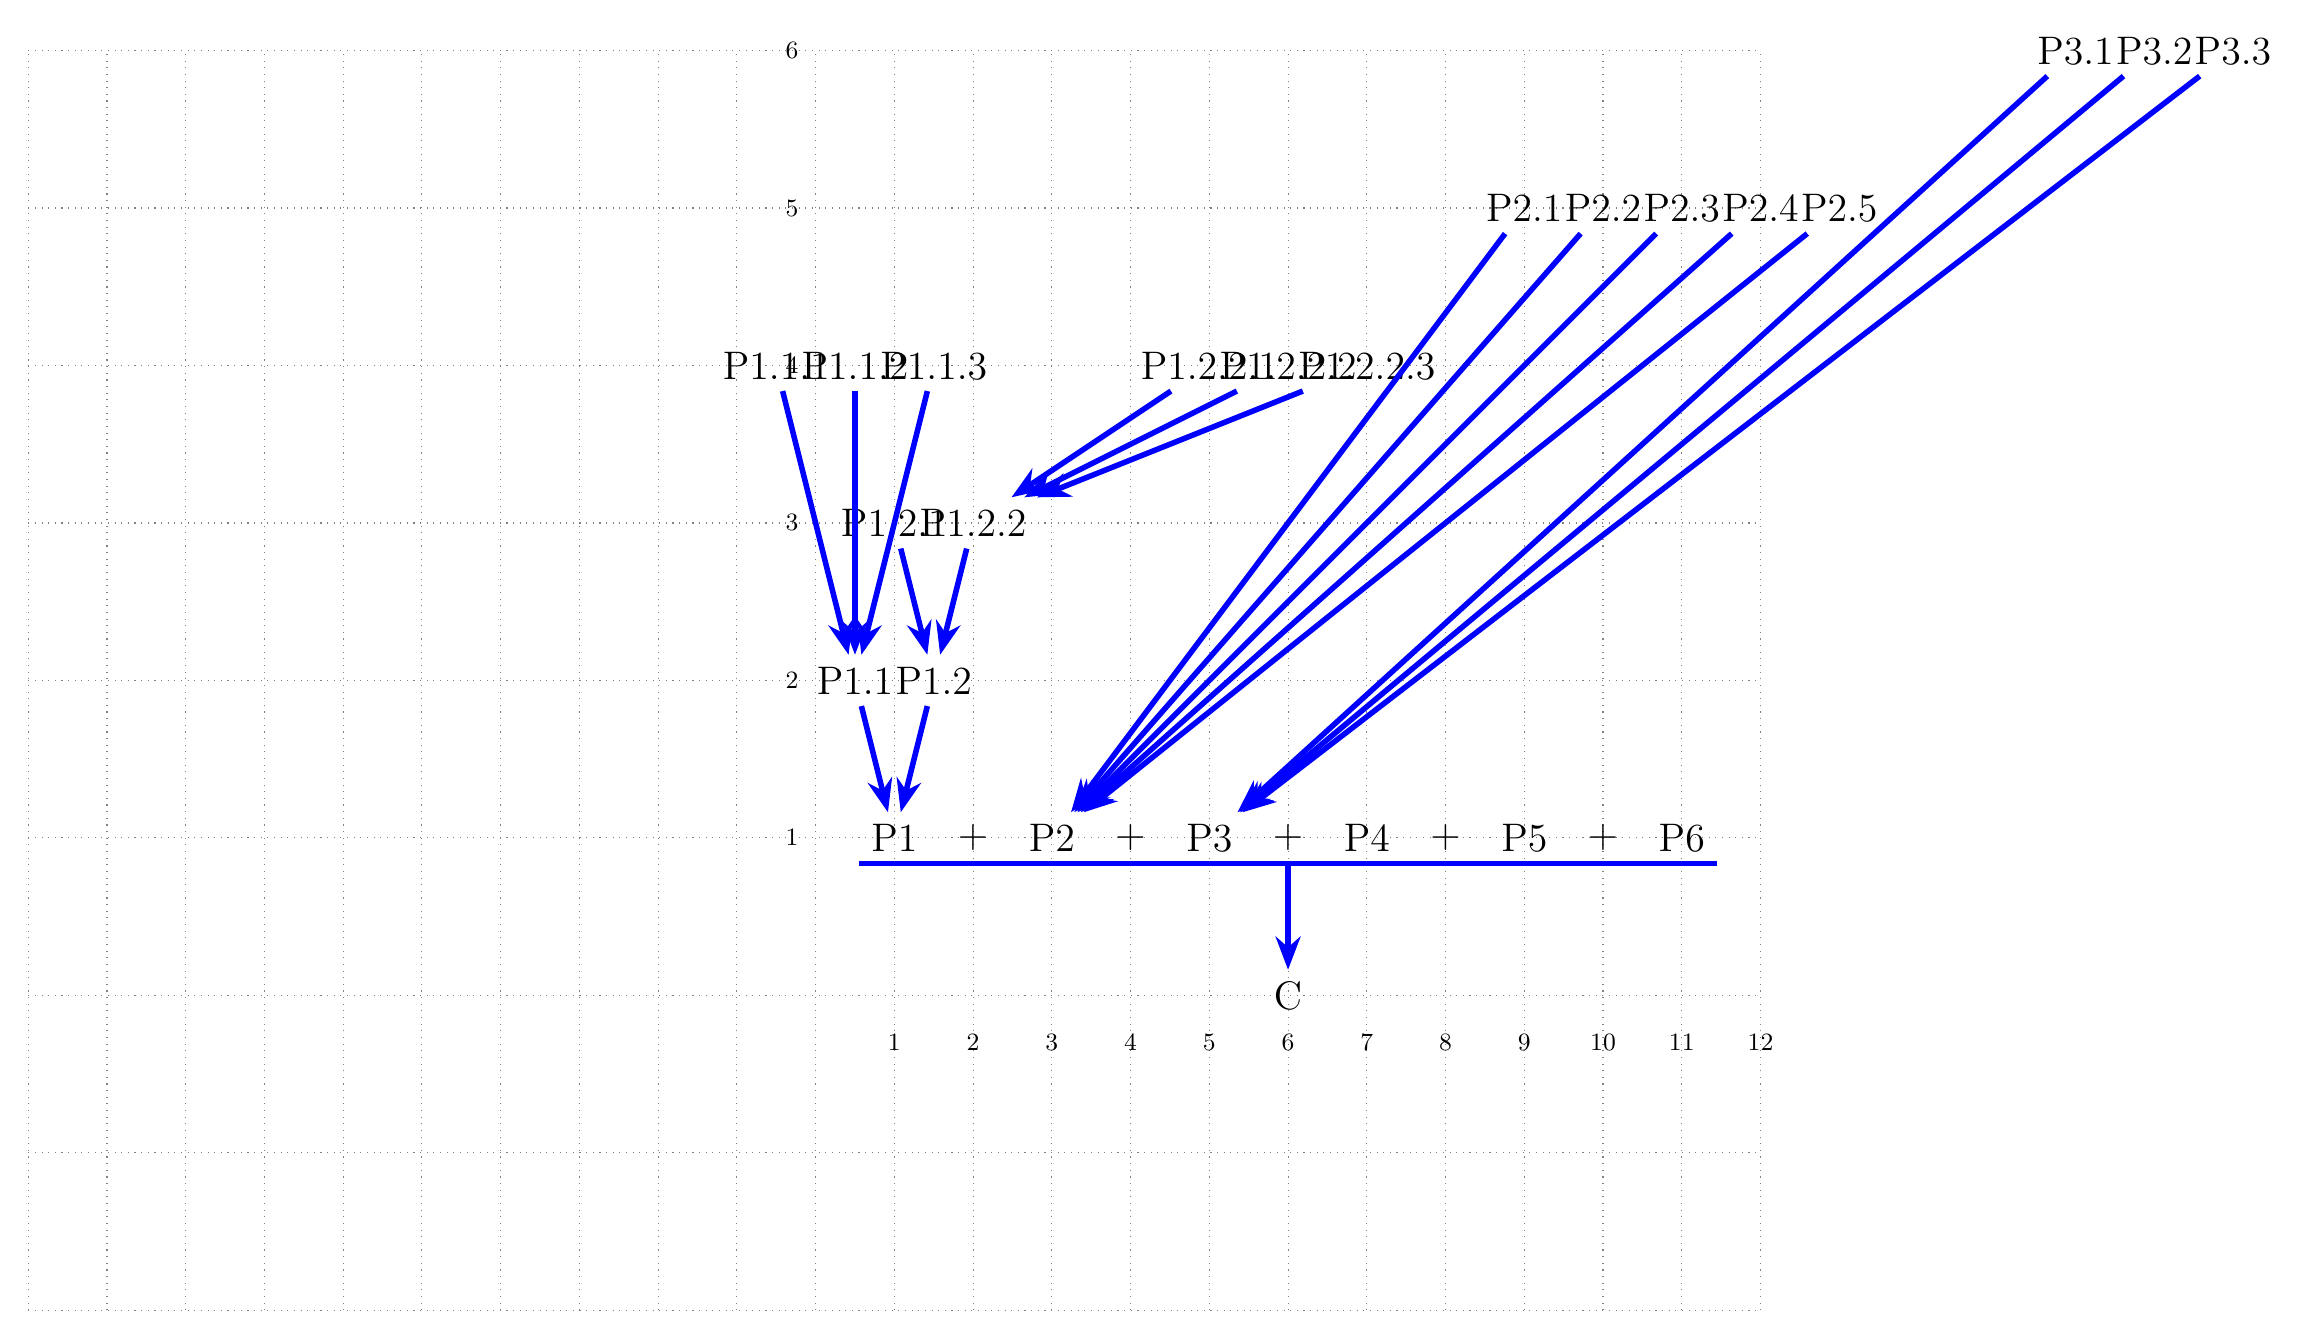
\begin{tikzpicture}[
	>=Stealth, 
	line width=2pt, 
	x=1.00cm,y=2.0cm, 
	font=\fontsize{14}{14}\selectfont
	]
	% begin grid
\draw[step=1, gray, thin, dotted] (-10,-2) grid (12,6);

% Grid numbers
\foreach \x in {1,2,3,4,5,6,7,8,9,10,11,12}
\node at (\x, -0.3) {\small \x};
\foreach \y in {1,2,3,4,5,6}
\node at (-0.3, \y) {\small \y};

% end grid
 

			\node (p3_1_16_6)   at (16.0, 6) {P3.1};
			\node (p3_2_17_6)   at (17.0, 6) {P3.2};
			\node (p3_3_18_6)   at (18.0, 6) {P3.3};
			\node (p2_1_9_5)   at (9.0, 5) {P2.1};
			\node (p2_2_10_5)   at (10.0, 5) {P2.2};
			\node (p2_3_11_5)   at (11.0, 5) {P2.3};
			\node (p2_4_12_5)   at (12.0, 5) {P2.4};
			\node (p2_5_13_5)   at (13.0, 5) {P2.5};
			\node (p1_1_1_0_4)   at (-0.5, 4) {P1.1.1};
			\node (p1_1_2_0_4)   at (0.5, 4) {P1.1.2};
			\node (p1_1_3_1_4)   at (1.5, 4) {P1.1.3};
			\node (p1_2_2_1_5_4)   at (5.0, 4) {P1.2.2.1};
			\node (p1_2_2_2_6_4)   at (6.0, 4) {P1.2.2.2};
			\node (p1_2_2_3_7_4)   at (7.0, 4) {P1.2.2.3};
			\node (p1_2_1_1_3)   at (1.0, 3) {P1.2.1};
			\node (p1_2_2_2_3)   at (2.0, 3) {P1.2.2};
			\node (p1_1_0_2)   at (0.5, 2) {P1.1};
			\node (p1_2_1_2)   at (1.5, 2) {P1.2};
			\node (p1_1_1)   at (1.0, 1) {P1};
			\node (plus_2_1)   at (2.0, 1) {+};
			\node (p2_3_1)   at (3.0, 1) {P2};
			\node (plus_4_1)   at (4.0, 1) {+};
			\node (p3_5_1)   at (5.0, 1) {P3};
			\node (plus_6_1)   at (6.0, 1) {+};
			\node (p4_7_1)   at (7.0, 1) {P4};
			\node (plus_8_1)   at (8.0, 1) {+};
			\node (p5_9_1)   at (9.0, 1) {P5};
			\node (plus_10_1)   at (10.0, 1) {+};
			\node (p6_11_1)   at (11.0, 1) {P6};
			\node (c_6_0)   at (6.0, 0) {C};

			\draw[->, blue] (p1_2_2_1_5_4) -- (p1_2_2_2_3);
			\draw[->, blue] (p1_2_2_2_6_4) -- (p1_2_2_2_3);
			\draw[->, blue] (p1_2_2_3_7_4) -- (p1_2_2_2_3);
			\draw[->, blue] (p1_1_1_0_4) -- (p1_1_0_2);
			\draw[->, blue] (p1_1_2_0_4) -- (p1_1_0_2);
			\draw[->, blue] (p1_1_3_1_4) -- (p1_1_0_2);
			\draw[->, blue] (p1_2_1_1_3) -- (p1_2_1_2);
			\draw[->, blue] (p1_2_2_2_3) -- (p1_2_1_2);
			\draw[->, blue] (p1_1_0_2) -- (p1_1_1);
			\draw[->, blue] (p1_2_1_2) -- (p1_1_1);
			\draw[->, blue] (p2_1_9_5) -- (p2_3_1);
			\draw[->, blue] (p2_2_10_5) -- (p2_3_1);
			\draw[->, blue] (p2_3_11_5) -- (p2_3_1);
			\draw[->, blue] (p2_4_12_5) -- (p2_3_1);
			\draw[->, blue] (p2_5_13_5) -- (p2_3_1);
			\draw[->, blue] (p3_1_16_6) -- (p3_5_1);
			\draw[->, blue] (p3_2_17_6) -- (p3_5_1);
			\draw[->, blue] (p3_3_18_6) -- (p3_5_1);
			\draw[->, blue] (plus_6_1) -- (c_6_0);

			\draw[blue] (p1_1_1.south west) -- (p6_11_1.south east);

\end{tikzpicture}

\section{test}

Some text

\end{center}

\end{document}
